In this lecture, we study the query complexity of search for classical randomized algorithms.
We analyze random sampling, relate it to the coupon collector problem, state a lower bound
for randomized search algorithms using Yao's minmax principle, and introduce Chernoff bounds.

\section{Query Complexity for Search}

We are given an array of $n$ slots (\cref{fig:array}). The array can only be accessed through
\emph{queries}: a query to a slot $x$ returns the value $f(x)$. In the \emph{search} problem, the goal
is to find the slot $x$ such that
\[f(x) = 1.\]
The cost of an algorithm is its \emph{query complexity}, i.e., the number of queries that it makes.

\begin{figure}[ht]
    \centering
    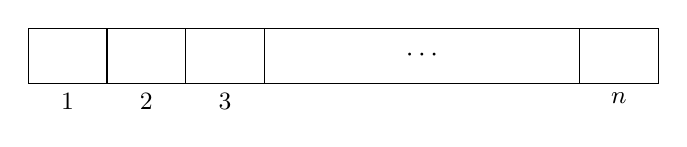
\begin{tikzpicture}
        \draw (0,0) rectangle (8,0.7);
        \foreach \x in {1,2,3,7} {\draw (\x,0) -- (\x,0.7);}
        \node at (5,0.35) {$\cdots$};
        \node[below] at (0.5,0) {\small $1$};
        \node[below] at (1.5,0) {\small $2$};
        \node[below] at (2.5,0) {\small $3$};
        \node[below] at (7.5,0) {\small $n$};
    \end{tikzpicture}
    \caption{An array of $n$ slots. We want to find the slot $x$ with $f(x) = 1$.}
    \label{fig:array}
\end{figure}

\subsection{Monte Carlo and Las Vegas Algorithms}

\begin{definition}[Monte Carlo and Las Vegas Algorithms]
    A \textbf{Monte Carlo} algorithm is a randomized algorithm whose error probability is $> 0$.

    A \textbf{Las Vegas} algorithm is a randomized algorithm whose error probability is $= 0$.
\end{definition}

\subsection{Random Sampling}

Consider random sampling \emph{with replacement}: in every step we query a slot that is chosen
uniformly at random among the $n$ slots. For every query,
\[\prob{\text{Success}} = \frac{1}{n}.\]
The number of queries until the first success is a \emph{geometric} random variable with
parameter $\sfrac{1}{n}$. Hence
\[\expectation{\text{queries}} = n.\]

If random sampling is stopped after a fixed number of queries, then it is a Monte Carlo algorithm,
since it can fail to find the slot. If we keep sampling until the slot is found, then it is a Las Vegas
algorithm, and
\[\expectation{\text{queries until find}} = n.\]

\section{Coupon Collector Problem}

Suppose that we want to distinguish 2 binary arrays (\cref{fig:binaryarrays}). To do this with
random sampling, all the $n$ slots have to be accessed. The number of queries needed by random sampling
(with replacement) to access all the $n$ slots is the \emph{coupon collector problem}.
We show that
\[\expectation{\text{queries}} \leq \bigO{n \log n}
    \quad\text{and}\quad
    \expectation{\text{queries}} \geq \bigOm{n \log n},\]
i.e., $\expectation{\text{queries}} = \bigTh{n \log n}$.

\begin{figure}[ht]
    \centering
    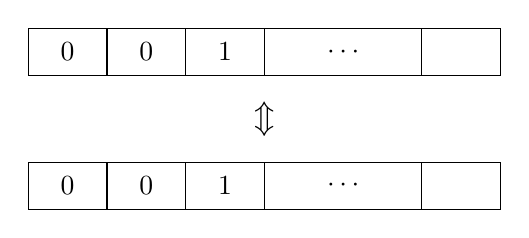
\begin{tikzpicture}
        % first array
        \draw (0,1.7) rectangle (6,2.3);
        \foreach \x in {1,2,3,5} {\draw (\x,1.7) -- (\x,2.3);}
        \node at (0.5,2.0) {$0$};
        \node at (1.5,2.0) {$0$};
        \node at (2.5,2.0) {$1$};
        \node at (4,2.0) {$\cdots$};
        % arrow between the arrays
        \node at (3,1.15) {\large $\Updownarrow$};
        % second array
        \draw (0,0) rectangle (6,0.6);
        \foreach \x in {1,2,3,5} {\draw (\x,0) -- (\x,0.6);}
        \node at (0.5,0.3) {$0$};
        \node at (1.5,0.3) {$0$};
        \node at (2.5,0.3) {$1$};
        \node at (4,0.3) {$\cdots$};
    \end{tikzpicture}
    \caption{To distinguish 2 binary arrays.}
    \label{fig:binaryarrays}
\end{figure}

\begin{theorem}[Coupon Collector]\label{thm:coupon}
    Let $X$ be the number of queries made by random sampling (with replacement) until all the
    $n$ slots are accessed. Then
    \[\expectation{X} = n H_n = \bigTh{n \log n},\]
    where $H_n = \sum_{i=1}^{n} \frac{1}{i}$ is the $\nth{n}$ harmonic number.
\end{theorem}

\begin{proof}
    Write
    \[X = X_1 + X_2 + \dots + X_n,\]
    where $X_i$ is the number of queries made to access a new slot, after $i-1$ different slots
    have already been accessed. When $i-1$ slots have been accessed, a query accesses a new slot
    with probability $\frac{n-(i-1)}{n}$. Hence $X_i$ is a geometric random variable,
    \[X_i \sim G\left(\frac{n-(i-1)}{n}\right),
        \qquad
        \expectation{X_i} = \frac{n}{n-(i-1)}.\]
    By linearity of expectation,
    \begin{align*}
        \expectation{X}
         & = \expectation{X_1 + X_2 + \dots + X_n} \\
         & = \sum_{i=1}^{n} \expectation{X_i}      \\
         & = \sum_{i=1}^{n} \frac{n}{n-(i-1)}      \\
         & = n \sum_{i=1}^{n} \frac{1}{n-i+1}      \\
         & = n H_n.
    \end{align*}
    Since $H_n = \bigTh{\log n}$, we get $\expectation{X} = \bigTh{n \log n}$.
\end{proof}

\newpage
\section{High Probability Bound}

The following was given in class as an exercise.

% Dashed box in my notes: exercise given in class.
\begin{exercise}
    Show that
    \[\prob{\text{any slot is accessed} \leq c \log n \text{ times}} \leq \frac{1}{n^2}.\]
\end{exercise}
\solutionspace % TODO: replace with \begin{proof} ... \end{proof}

The expectation of the number of queries is $\bigTh{n \log n}$. We now show that
$3 n \log n$ queries are enough with high probability. Here $\log$ is the natural logarithm.

\begin{theorem}\label{thm:whp}
    If random sampling makes $3 n \log n$ queries, then
    \[\prob{\text{fail}} \leq \frac{1}{n^2},
        \qquad\text{i.e.,}\qquad
        \prob{\text{Success}} \geq 1 - \frac{1}{n^2},\]
    where ``fail'' means that some slot is not accessed.
\end{theorem}

\begin{proof}
    Let $B_i$ be the event that slot $i$ is not accessed. A query does not access slot $i$ with
    probability $1 - \frac{1}{n}$. Using $1 - x \leq e^{-x}$,
    \begin{align*}
        \prob{B_i} = \prob{\text{slot $i$ not accessed}}
         & \leq \left(1 - \frac{1}{n}\right)^{3 n \log n} \\
         & \leq e^{-\frac{1}{n} \cdot 3 n \log n}         \\
         & = e^{-3 \ln n}                                  \\
         & = \frac{1}{n^3}.
    \end{align*}
    By the union bound,
    \[\prob{\bigcup_{i} B_i} \leq \sum_{i=1}^{n} \prob{B_i} = \frac{n}{n^3} = \frac{1}{n^2}.\]
\end{proof}

\section{Lower Bound for Randomized Algorithms}

\begin{theorem}\label{thm:lowerbound}
    Any Las Vegas randomized algorithm for search needs $\bigOm{n}$ expected queries.
\end{theorem}

The lower bound is shown using Yao's minmax principle.

\subsection*{Yao's Minmax Principle}

Let $A^{\mathrm{rand}}$ be a randomized algorithm, and let $\expectation{A^{\mathrm{rand}}}$ be its
expected number of queries. Let $\mu$ be a probability distribution over the inputs, and let
$D^{\mathrm{best}}_{\mu}$ be the best deterministic algorithm for inputs that are chosen according
to $\mu$. Then
\[\expectation{A^{\mathrm{rand}}}
    \geq \max_{\mu} \operatorname{\mathbb{E}}_{\mu}\left[D^{\mathrm{best}}_{\mu}\right]
    \geq \bigOm{n}.\]
The quantity $\operatorname{\mathbb{E}}_{\mu}\left[D^{\mathrm{best}}_{\mu}\right]$ is called the
\emph{distributional complexity}.

\section{Chernoff Bounds}

Let's say that a coin gives heads ($H$) with probability $\frac{1}{2} + \eps$ and tails ($T$) with
probability $\frac{1}{2} - \eps$. If we toss the coin $n$ times, then
\[\expectation{\text{Heads}} = n\left(\frac{1}{2} + \eps\right) = \frac{n}{2} + n\eps.\]
Chernoff bounds show that the number of heads is close to its expectation, so that
\[\prob{\text{Heads} < \frac{n}{2}} \sim \text{very small}.\]

In general, let
\[X = \sum_{i=1}^{n} X_i,
    \qquad
    X_i = \begin{cases}
        1 & \text{with probability } p_i,     \\
        0 & \text{with probability } 1 - p_i,
    \end{cases}\]
where the $X_i$ are independent Bernoulli random variables. If $p_i = p$ for all $i$, then
\[\expectation{X} = np, \qquad \variance{X} = np(1-p).\]
The distribution of $X$ is concentrated around its mean $np$ (\cref{fig:concentration}).

\begin{figure}[ht]
    \centering
    \begin{tikzpicture}
        % axes
        \draw[->] (-0.3,0) -- (8,0);
        \draw[->] (0,-0.2) -- (0,3.2);
        % distribution of X
        \draw[thick, domain=0:7.5, smooth, samples=120]
        plot (\x, {2.6*exp(-(\x-1.5)*(\x-1.5)/1.3)});
        % ticks
        \foreach \x/\l in {0.5/{\frac{1}{3}np}, 1.5/{np}, 4.5/{3np}, 7.5/{n}} {
                \draw (\x,0.08) -- (\x,-0.08) node[below] {\small $\l$};
            }
        \node[below left] at (0,0) {\small $0$};
        \draw[dashed] (4.5,0) -- (4.5,1.2);
    \end{tikzpicture}
    \caption{The distribution of $X$ is concentrated around the mean $np$.}
    \label{fig:concentration}
\end{figure}

\begin{theorem}[Chernoff Bounds]\label{thm:chernoff-0901}
    Let $X = \sum_{i=1}^{n} X_i$ be as above and let $\mu = \expectation{X}$.
    \begin{itemize}
        \item Upper tail (UI): for $0 < \delta < 1$,
              \[\prob{X \geq (1+\delta)\mu} \leq e^{-\frac{\mu \delta^2}{3}}.\]
        \item For $R \geq 6\mu$,
              \[\prob{X \geq R} \leq \frac{1}{2^R}.\]
        \item Lower tail (LI): for $0 < \delta < 1$,
              \[\prob{X \leq (1-\delta)\mu} \leq e^{-\frac{\mu \delta^2}{2}}.\]
    \end{itemize}
\end{theorem}
